\section{Three-tank Water Tank}
\label{sec:threetank}
%\fbox{LIU: OpenModelica Watertanks not available.}


\subsection{Example Description}
\label{sec:threetank_desc}

The three-tank water tank model is based upon a standard 20-sim example, and is developed to explore the impact on accuracy of multi-modelling across multiple CT models. The example comprises three water tanks which are filled and emptied. The first tank is filled from a source with a valve which may be turned on and off. The outflow of the first tank constitutes the inflow of the second, and so forth. A controller monitors the level of the third tank and controls a valve to a drain. 

A key feature of this example is the close coupling required between water tank 1 and 2, and the loose coupling to water tank 3. Water tanks 1 and 2 are tall and thin and are connected by a pipe at the bottom of the tanks (a diagram of the example is shown in Figure~\ref{fig:threetankoverview}), and therefore changes to the level of water tank 1 (due to water entering from the source) will quickly affect the level in water tank 2. This effect is not as prevalent between water tank 2 and 3. 


\begin{figure}[htbp]
\begin{center}
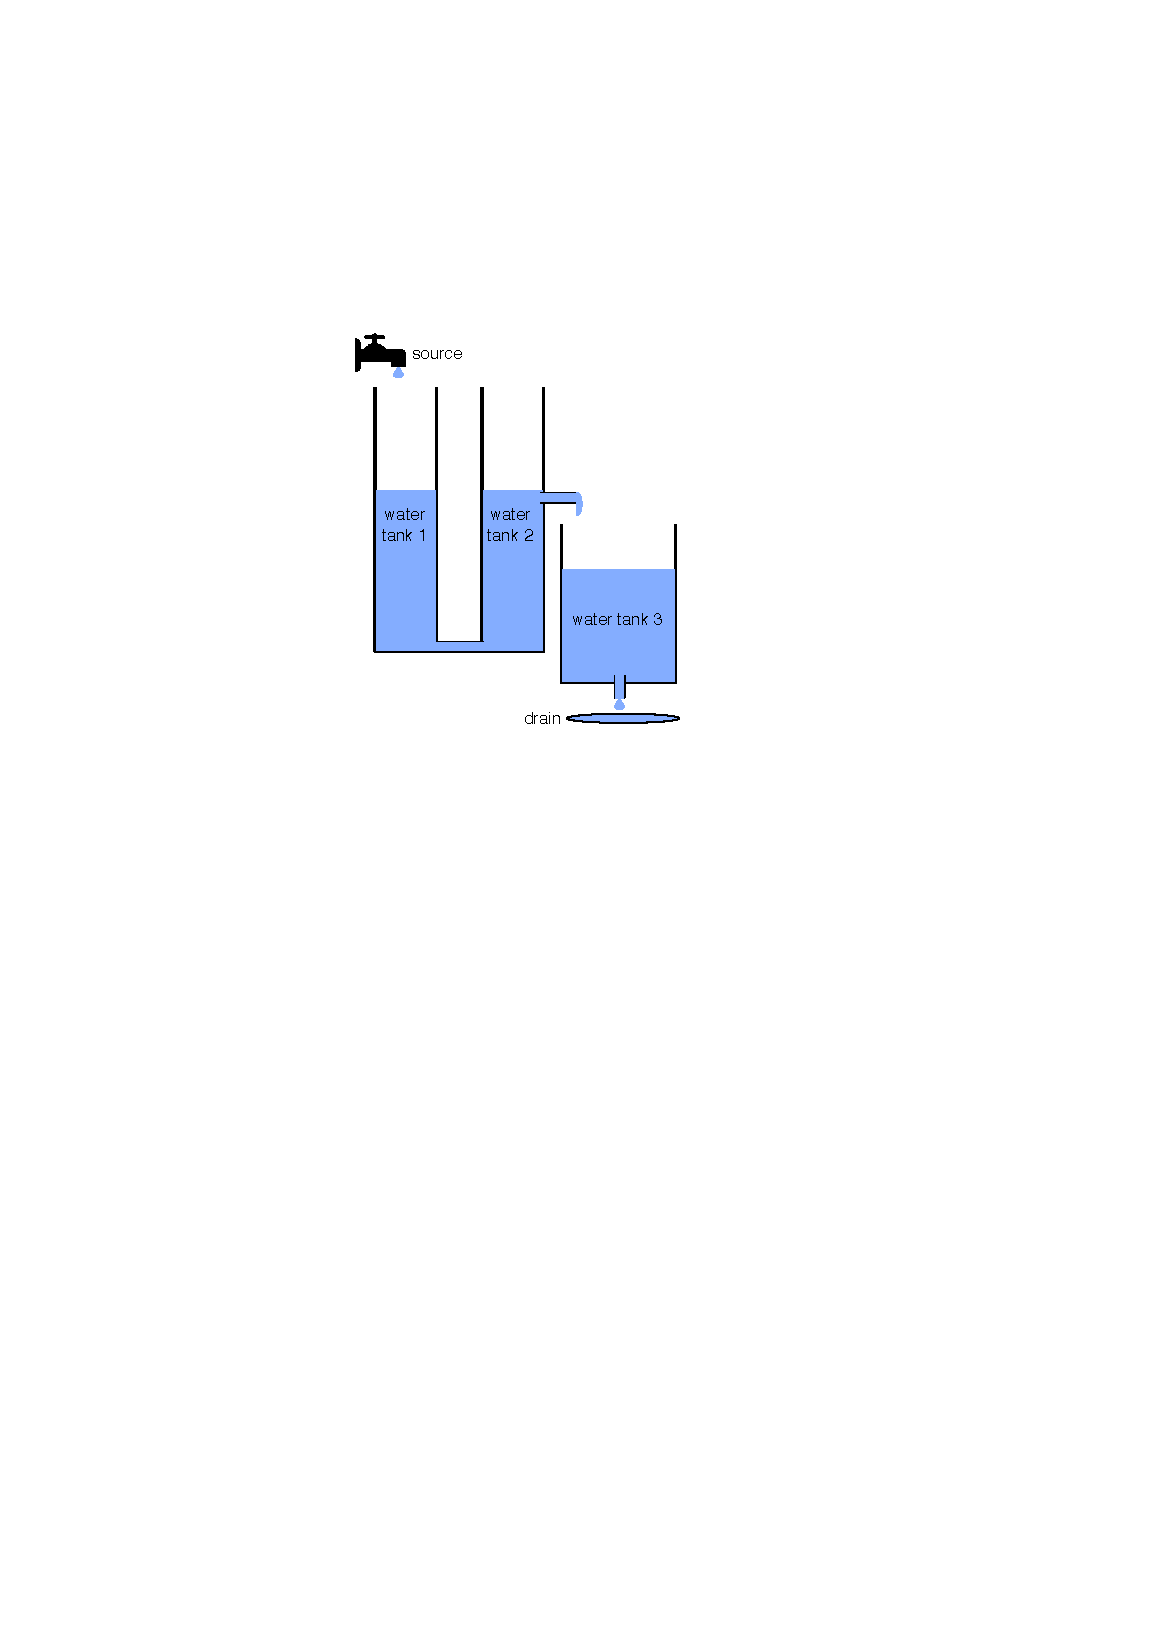
\includegraphics[width=0.5\textwidth]{threetank/ttwt_overview}
\caption{Overview of the three-tank water tank example}
\label{fig:threetankoverview}
\end{center}
\end{figure}

This pilot expands that in Section~\ref{sec:singletank}.

\subsection{Usage}
\label{sec:threetank_usage}

The example is available from the INTO-CPS application menu at \emph{File>Import Example Project} or at  \url{https://github.com/INTO-CPS-Association/example-three_tank_watertank} in the \emph{master} branch. There are several subfolders for the various elements: \texttt{DSEs} - contains work in progress DSE scripts; \texttt{FMU} -- contains the various FMUs of the study; \texttt{Models} -- contains the constituent models defined using the INTO-CPS simulation technologies; \texttt{Multi-models} -- contains the multi-model definitions and co-simulation configurations; \texttt{SysML} -- contains the SysML models defined for the study; resources -- various images for the purposes of this readme file. 

The \texttt{case-study\_three\_tank} folder can be opened in the INTO-CPS application to run the various co-simulations as detailed in this document. To run a simulation, expand one of the multi-models and click `Simulate' for an experiment. 


%\subsection{INTO-CPS Technology}
%\label{sec:threetank_into}
%
%We demonstrate the use of the INTO-CPS SysML profile in Section~\ref{sec:threetank_into_sys}. Based upon the design architecture defined using the SysML profile, a multi-model is constructed in Section~\ref{sec:threetank_into_mm} along with the defined connections. The study is also used to demonstrate the Co-Simulation Orchestration Engine (COE) in Section~\ref{sec:threetank_into_co}. % In Section~\ref{sec:threetank_3D} we outline the use of the INTO-SysML profile for visualisation of the model using a 20-sim FMU. 
%Section~\ref{sec:threetank_dse} outlines the use of the INTO-CPS DSE tool in the Three Tank model.

\subsection{INTO-CPS SysML profile}
\label{sec:threetank_into_sys}

A SysML model produced using the INTO-CPS profile comprises three diagrams and focusses on the structure of the water tank model for multi-modelling; an Architecture Structure Diagram and two Connections Diagrams. 

The Architecture Structure Diagram (ASD) in Figure~\ref{fig:threetankasd} shows the system composition in terms of component subsystems from the perspective of multi-modelling. As discussed in~\cite{INTOCPSD3.4}, this architecture differs from a holistic architecture due to the grouping of tanks into the different subsystems. 

\begin{figure}[htbp]
\begin{center}
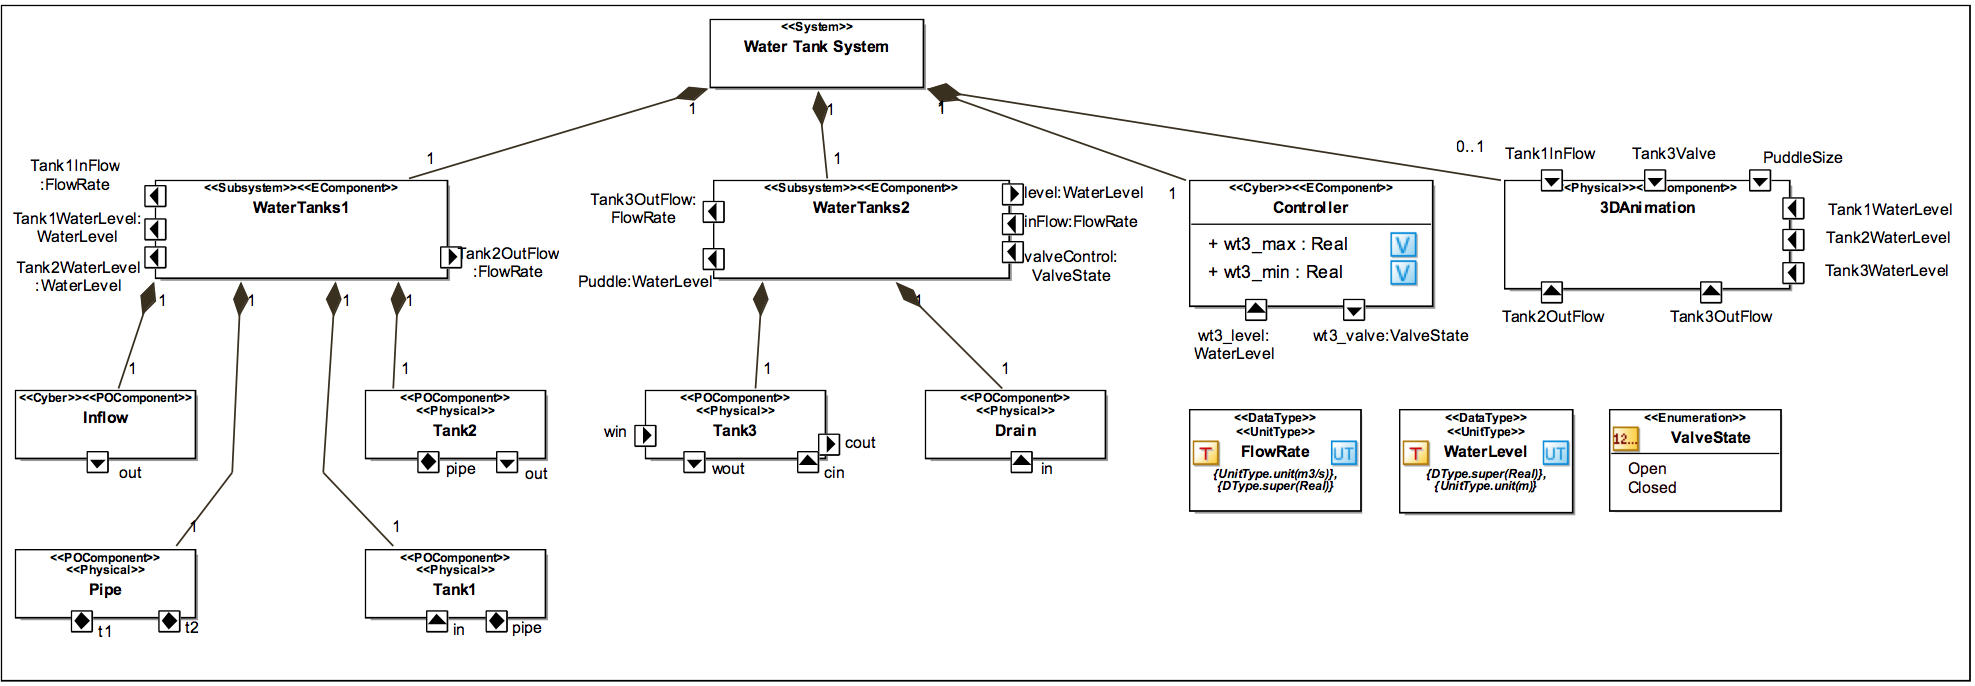
\includegraphics[width=1\textwidth]{threetank/ttwt_asd_vis.png}
\caption{Architecture Structure Diagram defining the Three-tank Water Tank system composition}
\label{fig:threetankasd}
\end{center}
\end{figure}

In this Water Tank system model, the water tanks are split between two subsystems: \emph{WaterTanks1} subsystem contains the \emph{Source}, two \emph{Water Tank} and  \emph{Pipe} components; \emph{WaterTanks2} subsystem comprises a single \emph{Water Tank} and \emph{Drain} components; a cyber component \emph{Controller} contains no other components; and the 3D component is available for visualising the behaviour of the system. 

To allow the visualisation FMU to depict the internal workings of the system's components, additional ports have been defined for the \emph{WaterTanks1} and  \emph{WaterTanks2} blocks. The \emph{WaterTanks1} component exposes: \texttt{Tank1InFlow} -- corresponding to the rate of water flowing into \emph{Tank1}; \texttt{Tank1WaterLevel} -- the water level of \emph{Tank1}; and \texttt{Tank2WaterLevel} -- the water level of \emph{Tank2}. The \emph{WaterTanks2} component exposes the additional ports: \texttt{Tank3OutFlow} -- corresponding to the rate of water flowing out of \emph{Tank3} and \texttt{puddle} -- the current volume of water in the drain (or puddle).

The two water tank subsystems are defined as continuous time models, both with 20-sim as the target platform. The controller component is a VDM-RT discrete event model. 

Two System Block Instances are defined in the model to represent alternative system configurations -- they are defined in separate Connections Diagrams (CDs). The CD in Figure~\ref{fig:threetankcd} defines connections as follows: at the subsystem-level,  the output of water from the \emph{WaterTanks1} subsystem is input to the \emph{WaterTanks2} subsystem. This subsystem has two connections with the \emph{Controller} cyber component - regarding the level and valve control.

\begin{figure}[htbp]
\begin{center}
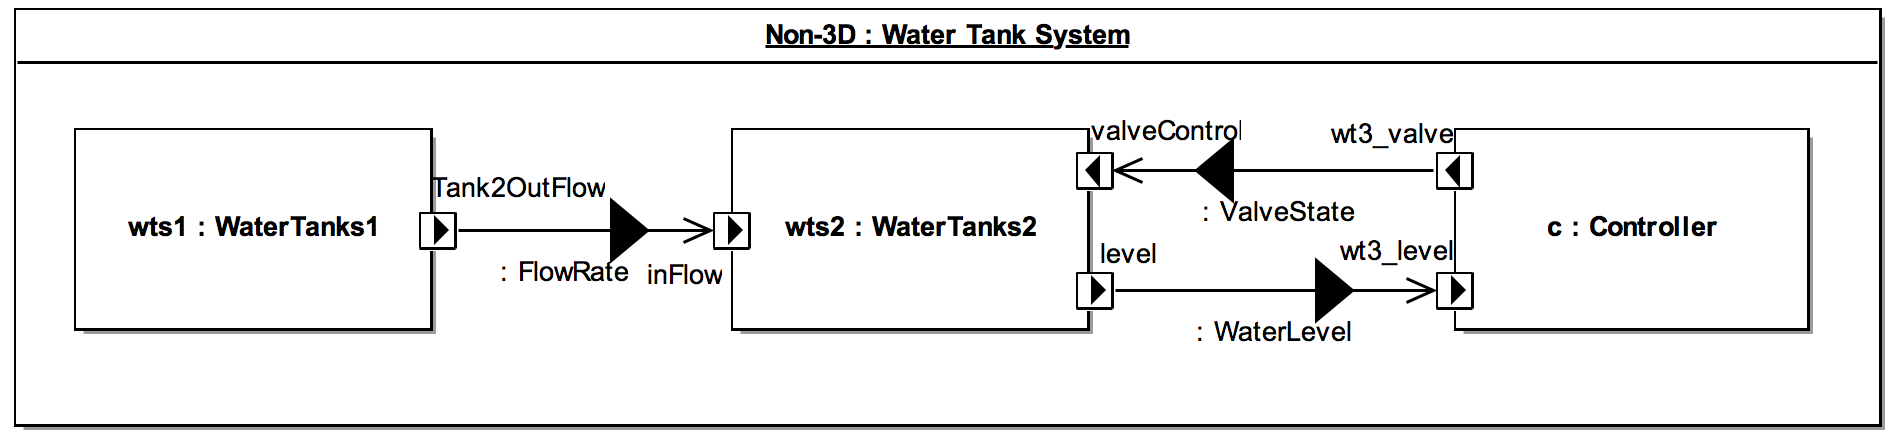
\includegraphics[width=0.85\textwidth]{threetank/ttwt_cd.png}
\caption{Connections Diagram defining the Three-tank Water Tank system connections}
\label{fig:threetankcd}
\end{center}
\end{figure}

 Figure~\ref{fig:threetankcdvis} depicts the second CD with several connectors between the system component instances and the 3D visualisation block instance. The connections in Figure~\ref{fig:threetankcd} are still present, with additional connections sending state information relating to tank water levels, flow rates and controller behaviour to the 3D model.
 
\begin{figure}[htbp]
\begin{center}
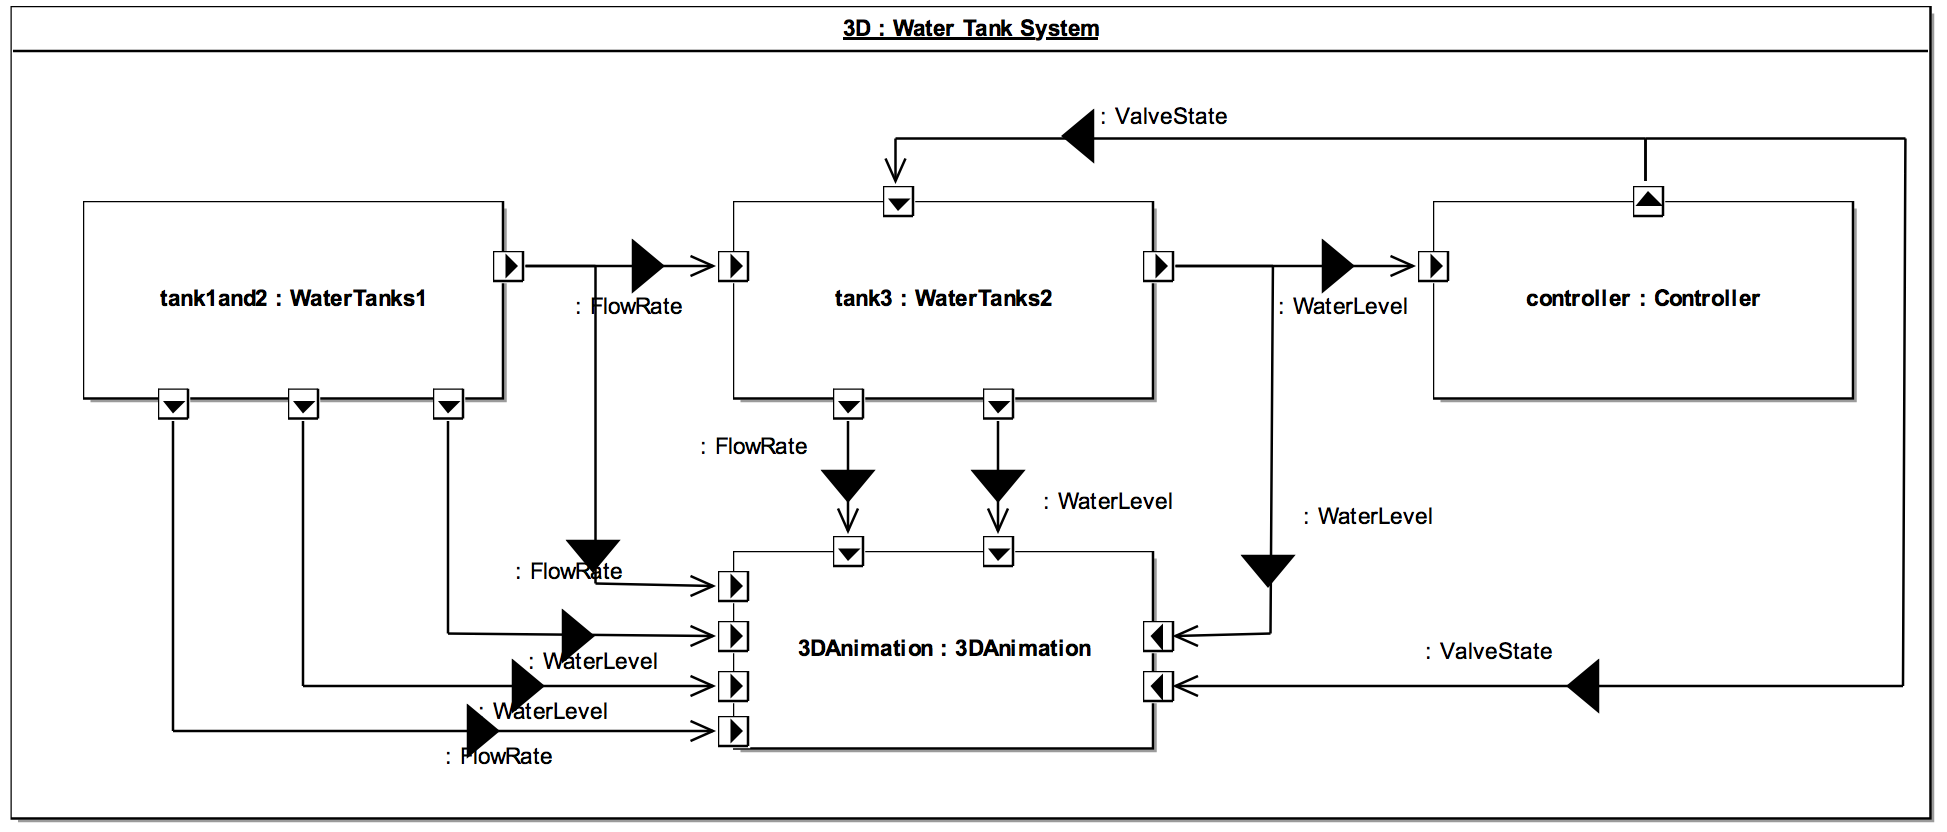
\includegraphics[width=0.85\textwidth]{threetank/ttwt_cd_vis.png}
\caption{Connections Diagram defining the Three-tank Water Tank system connections and elements for visualisation}
\label{fig:threetankcdvis}
\end{center}
\end{figure}

\subsection{Multi-model}
\label{sec:threetank_into_mm}

\subsubsection{Models}
\label{sec:threetank_into_models}

Given the ASD of the SysML model in  Section~\ref{sec:threetank_into_sys}, three (simulation) models are defined; two 20-sim subsystems and a VDM subsystem as shown in Figure~\ref{fig:threetankmm_ss}.

\begin{description}
\item[WaterTanks1, WaterTanks2] The partitioning of the 20-sim model is straightforward, with a single signal between the two 20-sim subsystems representing the flow of water between tanks 2 and 3. The rationale behind this split is that the flow rate between tank 1 and 2 has a high frequency and amplitude, suggesting that splitting the two tanks would result in erroneous results when time steps are imposed in co-simulation. 

\begin{figure}[htb!]
\begin{center}
\subfigure[Subsystems of Three-tank Water Tank multi-model]
{
     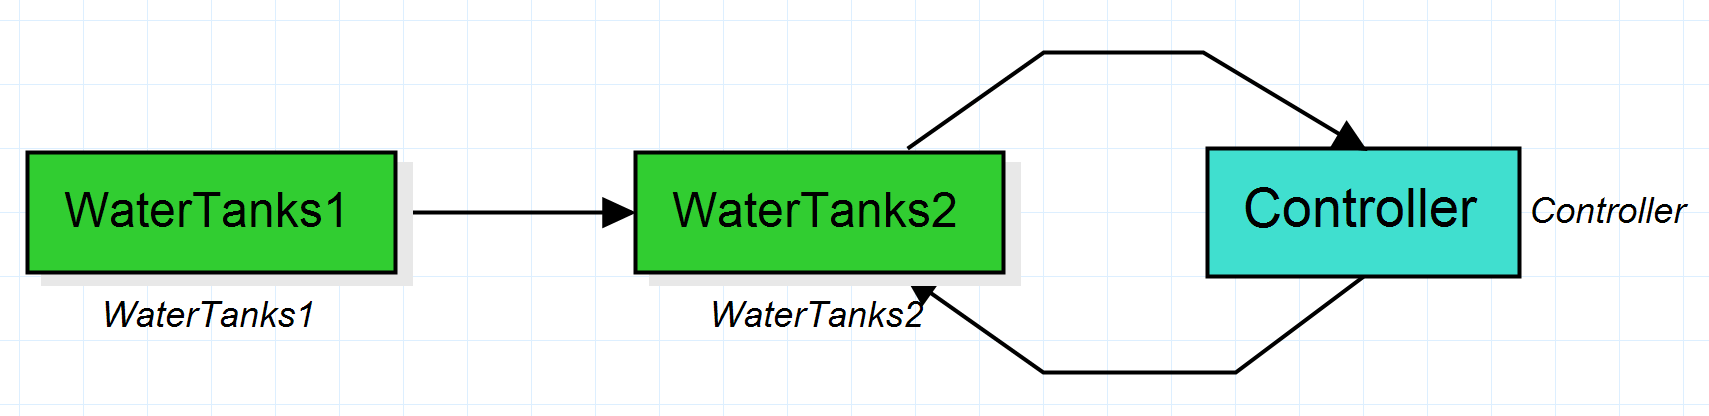
\includegraphics[width=0.6\linewidth]{threetank/ttwt_20sim_fmus} 
      \label{fig:threetankmm_ss}
}
\subfigure[WaterTanks1 subsystem]
{
     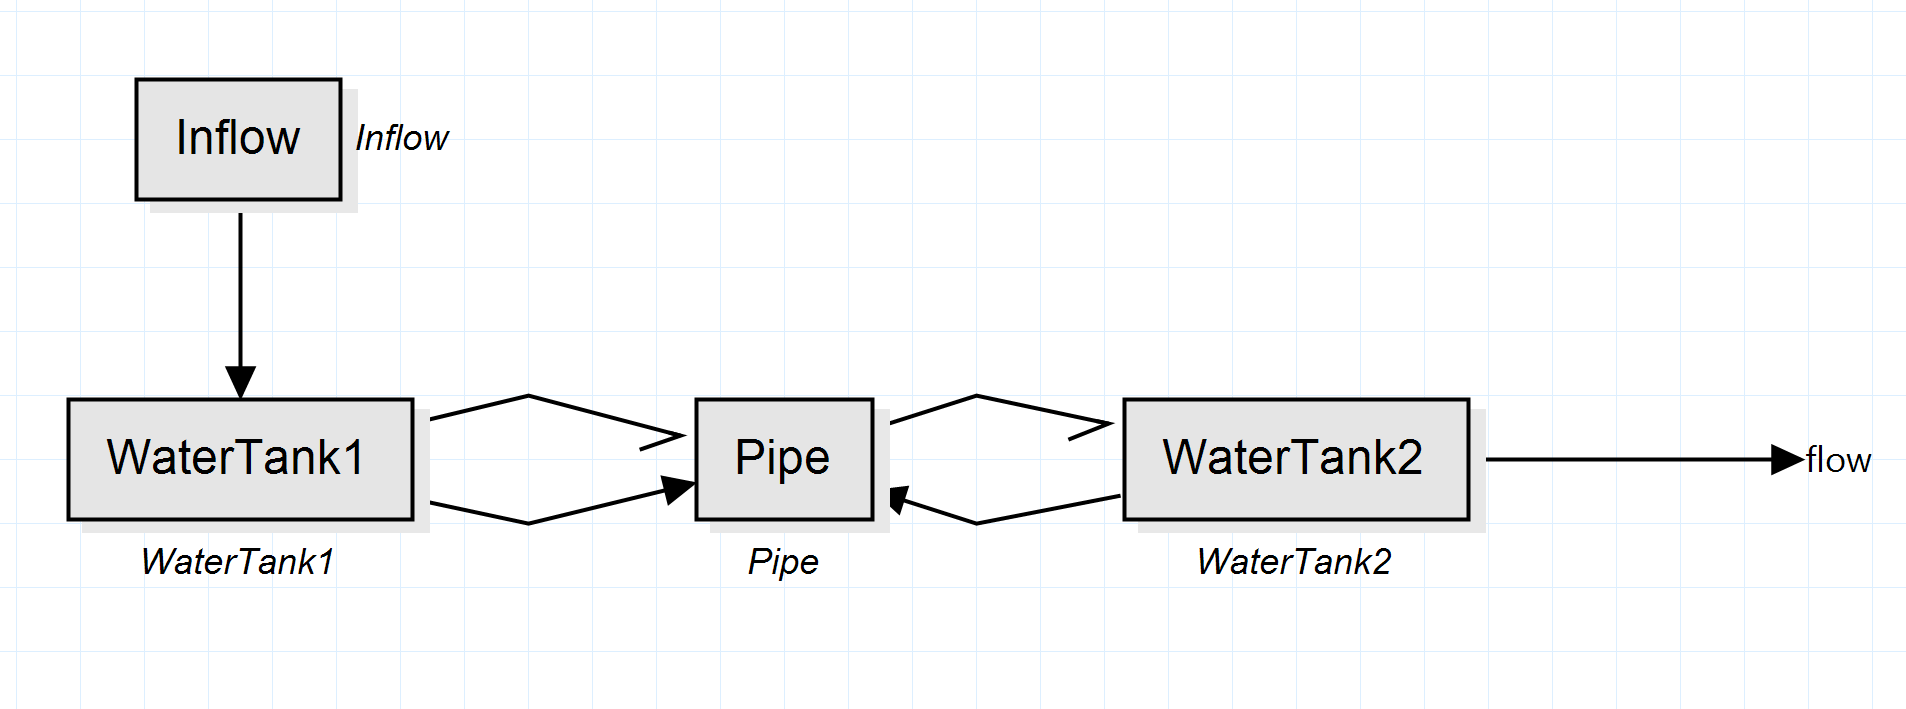
\includegraphics[width=0.6\linewidth]{threetank/ttwt_20sim_wt1fmu} 
      \label{fig:threetankmm_ss1}
}
\subfigure[WaterTanks2 subsystem]
{
     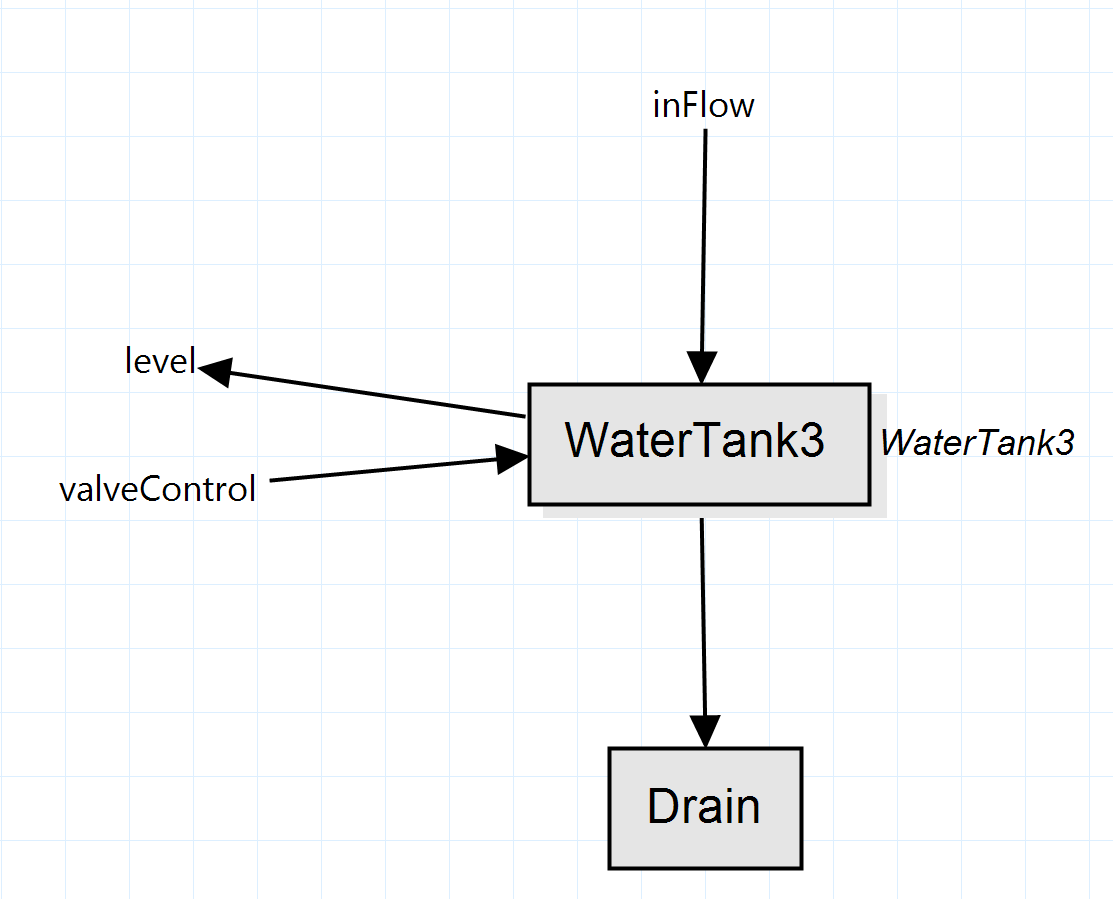
\includegraphics[width=0.35\linewidth]{threetank/ttwt_20sim_wt2fmu} 
      \label{fig:threetankmm_ss2}
}
\caption{20-sim models for the Three-tank Water Tank multi-model}
\label{fig:threetank_mm_20-sim}
\end{center}
\end{figure}

\item[Controller] The VDM-RT controller model is a simple controller, which governs \emph{Tank3}. The VDM-RT model contains a \emph{System} class containing \emph{HardwareInterface}  and \emph{Controller} objects -- \emph{hwi}  and \emph{controller}, respectively. The \emph{hwi} object includes the input and output variables of the model and design parameters. The \emph{controller} object is supplied with an instance of the \emph{LevelSensor}  (\emph{sensor}) and \emph{ValveActuator} (\emph{valve}) classes -- each given access to different parts of the \emph{hwi} object. The \emph{sensor} object represents the sensor that measures the current water level, and \emph{valve} is  represents the valve at the bottom of the tank.

The control loop retrieves the current level of water from the sensor and determines whether to set the valve to be open or closed depending on the level compared to some set maximum or minimum value. 
\end{description}

\subsubsection{Configuration}
\label{sec:threetank_into_mm}

Two multi-models are defined for the Three Tank Study corresponding to the two System block instances defined in the CDs of the SysML model in Section~\ref{sec:threetank_into_sys}. 

In the first multi-model (\emph{Non-3D}), there are three FMUs and three connections. The FMUs comprise: WaterTankController, threewatertank1 and threewatertank2 -- exported from the VDM-RT and 20-sim models described above. The connections are as follows: firstly between the \texttt{flow} port of \emph{WaterTanks1} to the \texttt{inFlow} of \emph{WaterTanks2}; secondly between \texttt{valveControl} port of the \emph{WaterTanks2} model to the \texttt{wt3\_valve} of the \emph{Controller}; and finally from the \texttt{wt3\_level} of the \emph{Controller} to the \texttt{level} port of \emph{WaterTanks2}. 

In addition, there are two \emph{design parameters} -- \texttt{wt3\_min} and \texttt{wt3\_max}, both of type \texttt{real}.

The complete configuration is given in Figure~\ref{fig:threetankconfig}.

\begin{figure}[htbp]
\begin{center}
\begin{config}
{		
	"fmus":{
		"{c}":"WaterTankController.fmu",
		"{t1}":"threewatertank1.fmu",
		"{t2}":"threewatertank2.fmu"
	},
	"connections":{
		"{c}.controller.wt3_valve":["{t2}.tank2.valveControl"],
		"{t1}.tank1.Tank2OutFlow":["{t2}.tank2.inFlow"],
		"{t2}.tank2.level":["{c}.controller.wt3_level"]
	},
	"parameters":{
		"{c}.controller.wt3_max":1.7,
		"{c}.controller.wt3_min":1.3
	}
}
\end{config}
\caption{Configuration file for Three-tank Water Tank system}
\label{fig:threetankconfig}
\end{center}
\end{figure}


The second multi-model (\emph{3D}) uses the 3D visualisation FMU, and has additional connections to that FMU, as shown in Figure~\ref{fig:threetankconfig2}.

\begin{figure}[htbp]
\begin{center}
\begin{config}
{
	"fmus":{
		"{c}":"WaterTankController.fmu",
		"{t1}":"threewatertank1.fmu",
		"{t2}":"threewatertank2.fmu",
		"{3d}":"3DAnimationFMU.fmu"
	},
	"connections":{
		"{c}.controller.wt3_valve":["{t2}.tank2.valveControl","{3d}.3DAnimationFMU.animation.tank3.valve.control"],
		"{t1}.tank1.Tank2OutFlow":["{t2}.tank2.inFlow","{3d}.3DAnimationFMU.animation.tank2.outflow"],
		"{t2}.tank2.level":["{c}.controller.wt3_level", "{3d}.3DAnimationFMU.animation.tank3.waterlevel"],
		"{t1}.tank1.Tank1InFlow":["{3d}.3DAnimationFMU.animation.tank1.inflow"],
		"{t1}.tank1.Tank1WaterLevel":["{3d}.3DAnimationFMU.animation.tank1.waterlevel"],
		"{t1}.tank1.Tank2WaterLevel":["{3d}.3DAnimationFMU.animation.tank2.waterlevel"],
		"{t2}.tank2.Tank3OutFlow":["{3d}.3DAnimationFMU.animation.tank3.outflow"],
		"{t2}.tank2.puddle":["{3d}.3DAnimationFMU.animation.drain.puddle"]
	},
	"parameters":{
		"{c}.controller.wt3_max":1.7,
		"{c}.controller.wt3_min":1.3
	}
}
\end{config}
\caption{Configuration file for Three-tank Water Tank system}
\label{fig:threetankconfig2}
\end{center}
\end{figure}

\subsection{Co-simulation}
\label{sec:threetank_into_co}

Using the INTO-CPS Co-simulation Engine (COE), we may simulate the three FMU multi-model. We are able to log the water level of tank 3 and the flow rate between tank 2 and 3. These values are shown in the graph in Figure~\ref{fig:threetankcoeres}, using a fixed step size of \emph{0.05}. A simulation time of at least 20 seconds is recommended so to observe changes in controller behaviour.

\begin{figure}[htbp]
\begin{center}
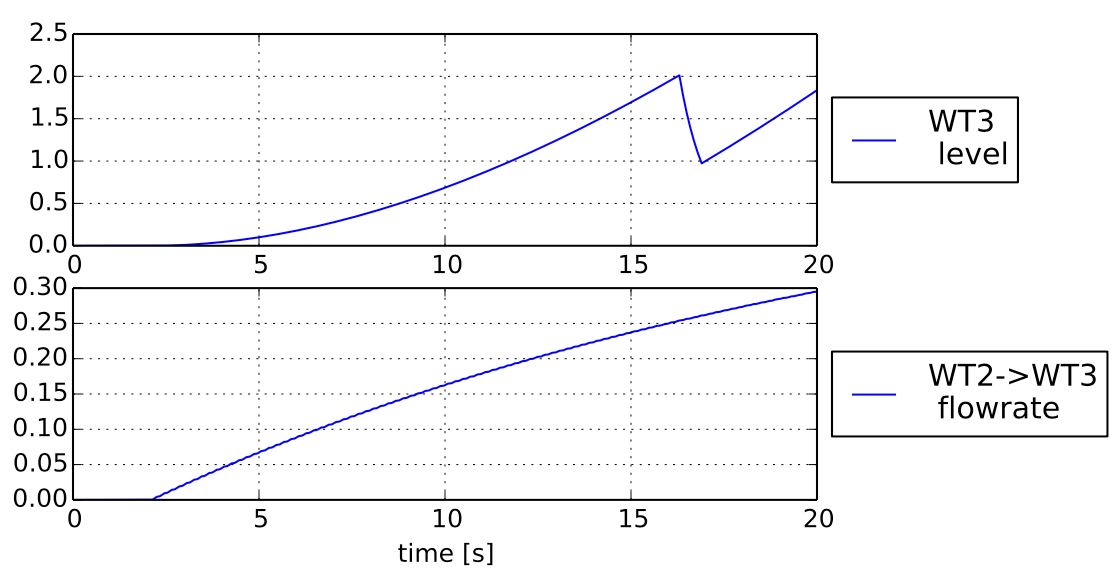
\includegraphics[width=0.85\textwidth]{threetank/ttwt_coe_res.png}
\caption{Simulation results using the INTO-CPS COE}
\label{fig:threetankcoeres}
\end{center}
\end{figure}

The results in the graph correspond closely to those of the baseline Crescendo model illustrated in~\cite{INTOCPSD3.4}. During simulation, the water level raised to the maximum value (2.0 meters) and at 16.3 seconds the tank 3 valve is opened by the VDM-RT controller and the level drops to just below the minimum (1.0 meters) and at 16.9 seconds the valve is closed and the water level begins to rise again.

Co-simulating the 3D multi-model opens a 3D visualisation window as shown in Figure~\ref{fig:threetank3d} which depicts the state of the Three-tank system as the simulation progresses. 

\begin{figure}[htbp]
\begin{center}
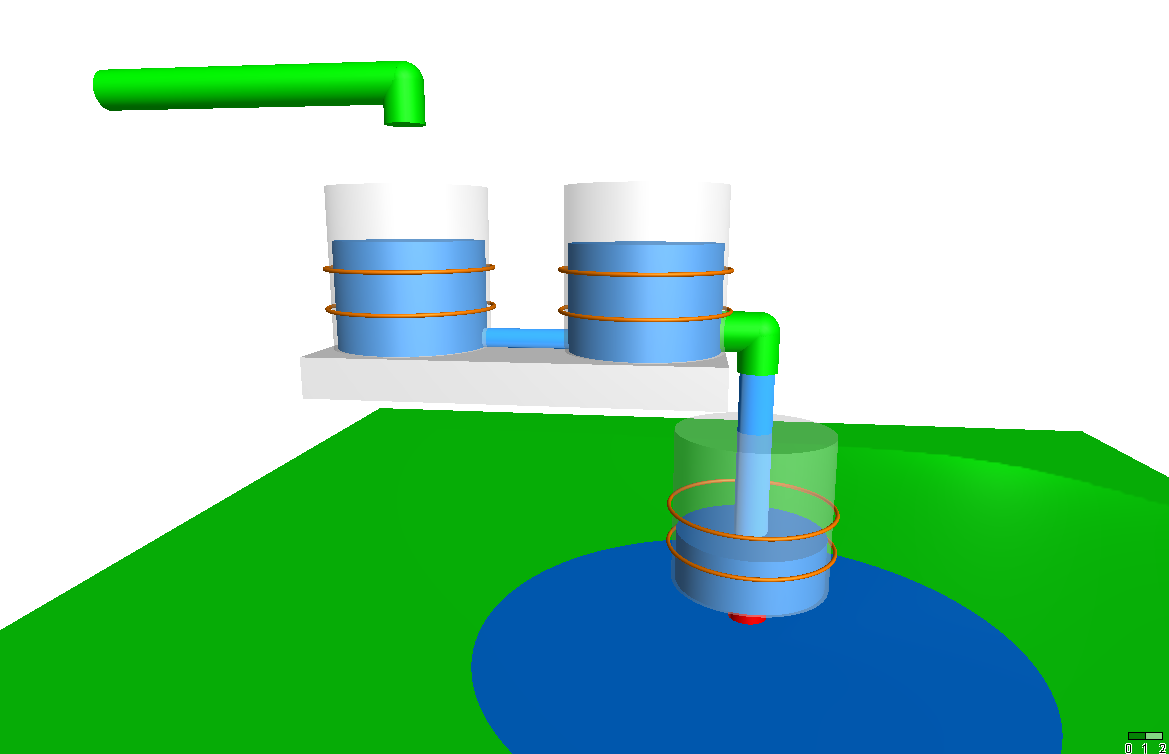
\includegraphics[width=0.75\textwidth]{threetank/TTWT_3D.png}
\caption{3D visualisation of the Three-tank Water Tank system}
\label{fig:threetank3d}
\end{center}
\end{figure}

\subsection{Analyses and Experiments}

\subsubsection{Design Space Exploration}
\label{sec:threetank_dse}

A simple DSE experiment is included in the project, which demonstrates the use of the DSE tool support. The experiment varies the two design parameters of the study -- \texttt{wt3\_min} and \texttt{wt3\_max}. These parameter values may be set between $0.2$ and $2.0$ in intervals of $0.2$. A constraint on the parameters (\texttt{{controller}.controller.wt3\_max $>$ {controller}.controller.wt3\_min}) ensures that the maximum water value is always larger than the minimum water level. 

Two objectives are defined: \textit{cumulativeDeviation} and \textit{vCount}. The first objective, \textit{cumulativeDeviation}, is to minimise the cumulative deviation from a desired level - set to $1.0$. The second objective, \textit{vCount}, is to minimise the number of valve operations -- i.e. have a lower number of valve state changes. The use of Pareto ranking, minimising both objectives gives the resultant graph in Figure~\ref{fig:threetankdse}.

\begin{figure}[h]
\begin{center}
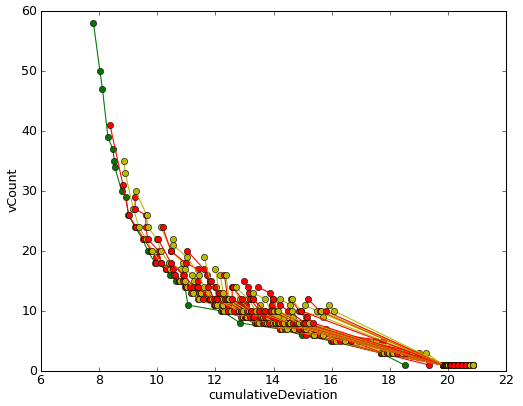
\includegraphics[width=0.75\textwidth]{threetank/dse_pareto_graph.png}
\caption{Design Space Exploration Pareto graph of the Three-tank Water Tank system}
\label{fig:threetankdse}
\end{center}
\end{figure}

From the results we see that there is a clear tradeoff to be made between levels which optimise  each objective -- it is for the engineer to determine which of these is more important. The green line on the graph (the left-most set of results) gives this `non-dominated' set of results -- also given as a table as in Figure~\ref{fig:threetankdsetable}. In broad terms the ranking shows: levels closer to the desired level (e.g. \texttt{wt3\_min} = $1.0$ and \texttt{wt3\_max} = $1.05$) produce results with a lower cumulative deviation, but higher valve operation count; and a minimum level further from the desired level (e.g. \texttt{wt3\_min} = $0.2$) produces results with a lower valve operation count, but higher cumulative deviation.

\begin{figure}[h]
\begin{center}
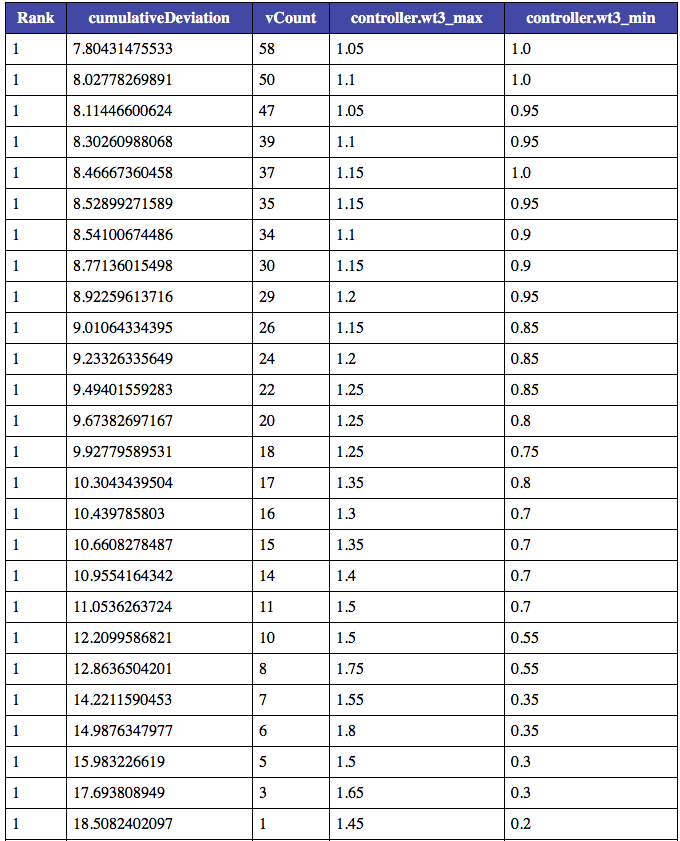
\includegraphics[width=0.75\textwidth]{threetank/dse_results_table_nds.png}
\caption{Design Space Exploration Pareto front table of the Three-tank Water Tank system}
\label{fig:threetankdsetable}
\end{center}
\end{figure}


\subsubsection{Test Automation}
\label{sec:threetank_ta}

\begin{figure}
\begin{center}  
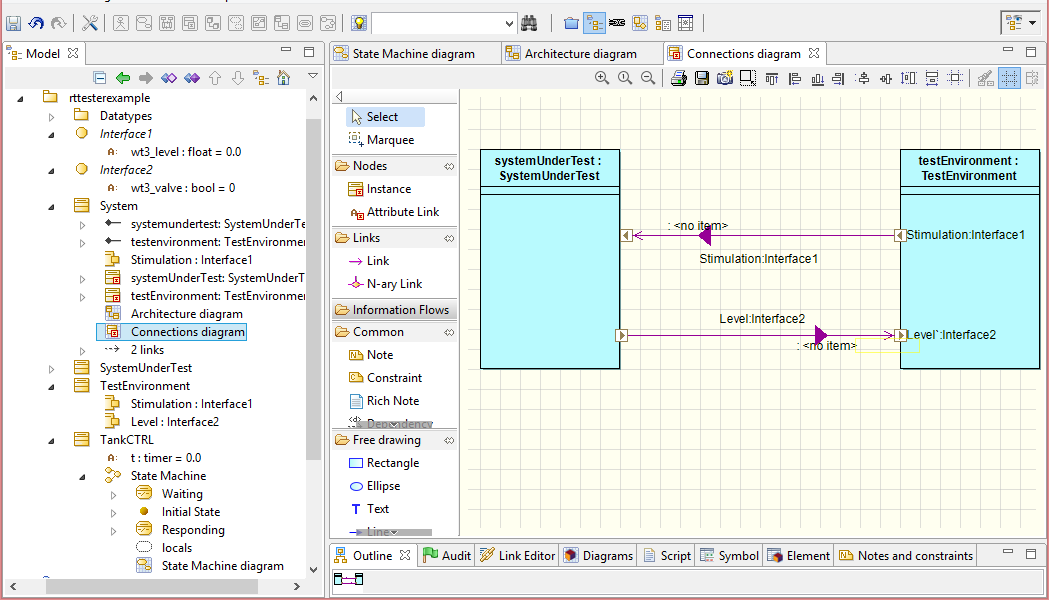
\includegraphics[width=\textwidth]{threetank/ta_overview}
\caption{Overview of the three-tank test model in Modelio}
\label{fig:threetanktestmodel}
\end{center}
\end{figure}

Test automation can also be applied to the controller of the three-tank example. A SysML model exists that
represents the test model for this system which can be used to produce tests for models and implementations of the
controller in RT-Tester\footnote{Note that this is a different SysML model used for the co-simulation multi-model.}. The model consists of a specified System Under Test (SUT), which in this case corresponds to
the controller, and the Test Environment (TE) which is the rest of the water tank system, but specifically the water
tank the controller is monitoring. A screen shot giving an overview of the test model is shown in
Figure~\ref{fig:threetanktestmodel}.

The  SUT and TE are specified using the blocks \emph{SystemUnderTest} and \emph{TestEnvironment}, respectively. The SUT
block an input flow port called \emph{Stimulation} of type \emph{Interface1} and an output port of type
\emph{Interface2}. The TE has the same ports but in the opposite direction. \emph{Interface1} specifies the shared
variables that the SUT will read from. In this case it consists of a single variable \emph{wt3\_level}, as seen on the
right, which corresponds to the FMU input. Likewise, \emph{Interface2} specifies the shared variable that the SUT will
write to, in this case the variable \emph{wt3\_valve} which gives the valve status. The two blocks are linked together
so that the SUT and TE can communicate on these channels.

\begin{figure}
\begin{center}  
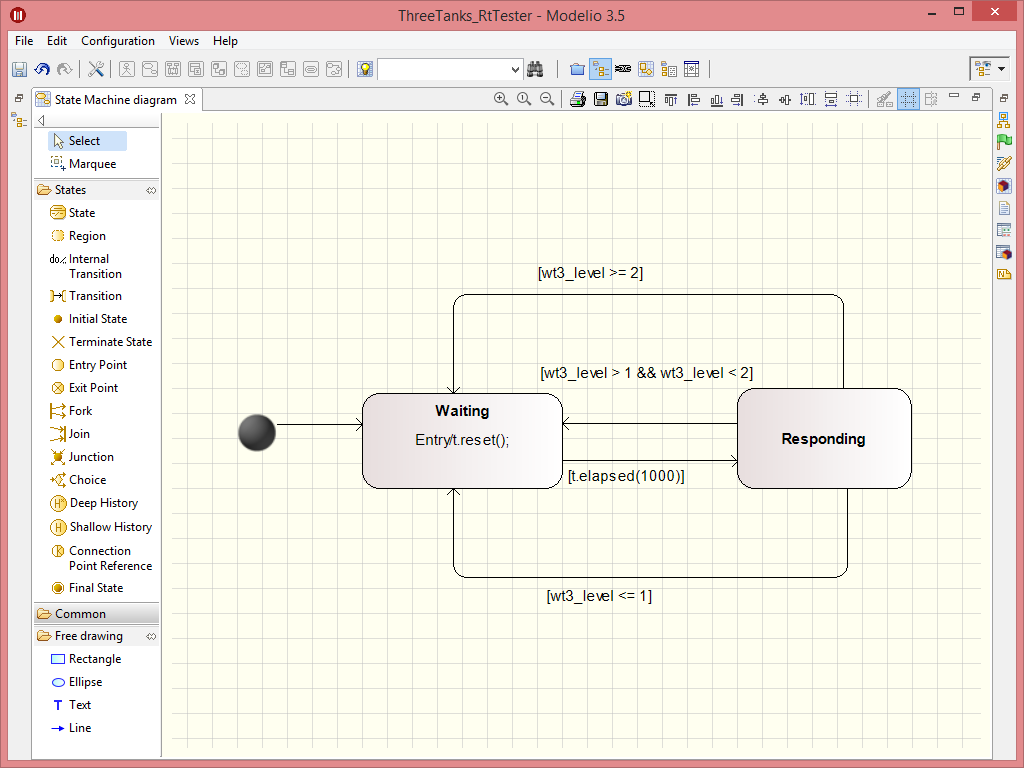
\includegraphics[width=\textwidth]{threetank/ta_state_machine}
\caption{State machine for abstract behaviour of three-tank controller}
\label{fig:threetankstatemachine}
\end{center}
\end{figure}

In order to generate tests it is necessary to specify an abstract model for the controllers behaviour, which should be
modelled using a timed state machine. We thus created the SysML state machine diagram shown in
Figure~\ref{fig:threetankstatemachine}. The three-tanks controller is relatively simple and so the state machine has
only two states. The \textbf{Waiting} state means that the controller is waiting until sufficient time has elapsed to
poll the sensors and act accordingly. It has a single outgoing transition with the guard \texttt{t.elapsed(1000)}. The
variable \texttt{t} is a timer for this state machine. It advances in time and can be checked and reset at certain
points, rather like a stop-watch. The state machine changes to the \textbf{Responding} state once 1000 ms (1 s) has
elapsed.

The \textbf{Responding} state contains the main decision logic for the controller. It has three outgoing edges with
guards and actions (the latter are not shown). If the water level polled on variable \emph{wt3\_level} remains within
the safe zone of between 1 and 2 then the state machine returns to state \textbf{Responding} with no action. If the
water level is greater than or equal to 2, the \emph{wt3\_valve} variable is set to 0 to shut off the valve, and the
controller returns to the \textbf{Waiting} state. Otherwise, if the level is less than or equal to 1, then the valve is
turned on by setting \emph{wt3\_valve} to 1.

\begin{figure}
  \begin{center}
    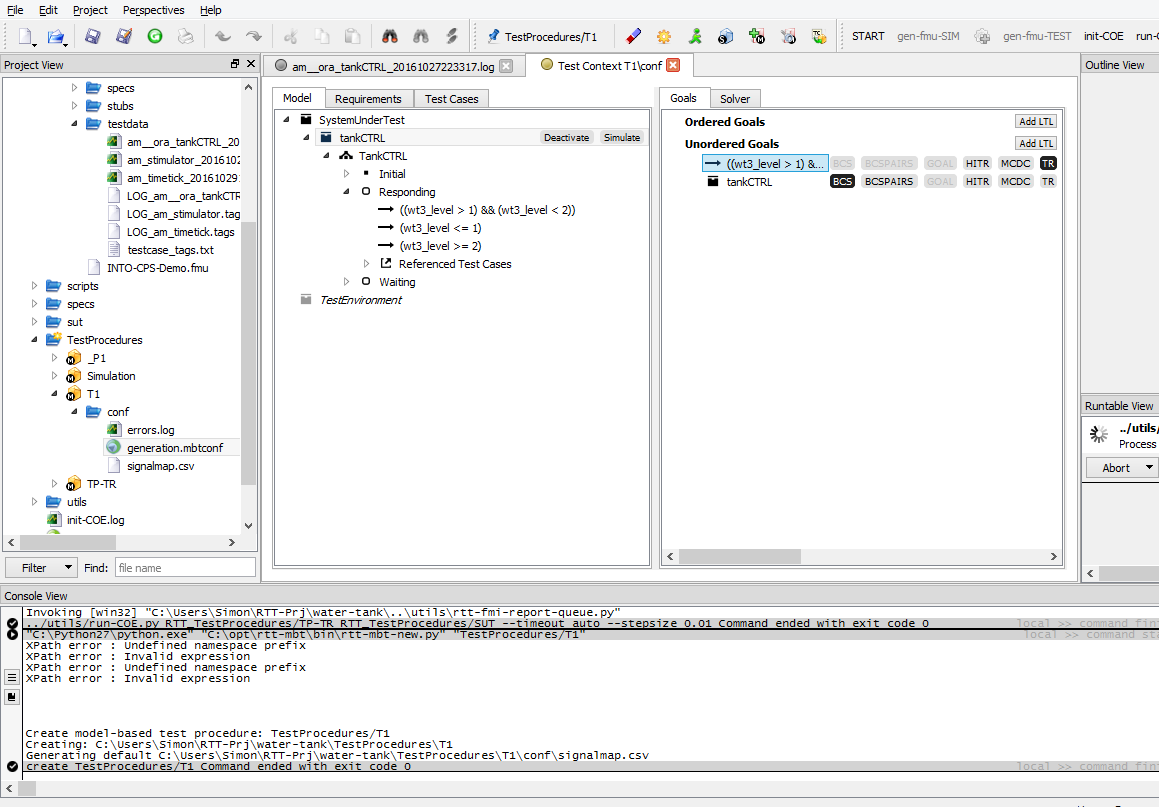
\includegraphics[width=16cm]{threetank/ta_rtt2.png}
  \end{center}
  \caption{Configuring a test procedure}
  \label{fig:ta-proc}
\end{figure}

This behavioural model must be input into RT-Tester to generate and execute tests. We do this by first exporting XMI from Modelio by
selecting the project name, and then the menu item \emph{Import / Export > Export > XMI export}. The model can then be
imported from RT-Tester by selecting \emph{Project > Model-based testing > Import model > Import from file}. This
currently must be done from the existing \emph{water-tanks} model available in RT-Tester to ensure that the FMU is
correctly set up. One of the standard test procedures can then be run, or a new test procedure can be created by
selecting \emph{New > MBT Test Procedure} and then using test procedure \texttt{TestProcedures/\_P1} as a
template. Suitable tests can be configured from the \emph{conf > generation.mbtconf} file in the new directory as
illustrated in Figure~\ref{fig:ta-proc}.

\begin{figure}
  \begin{center}
    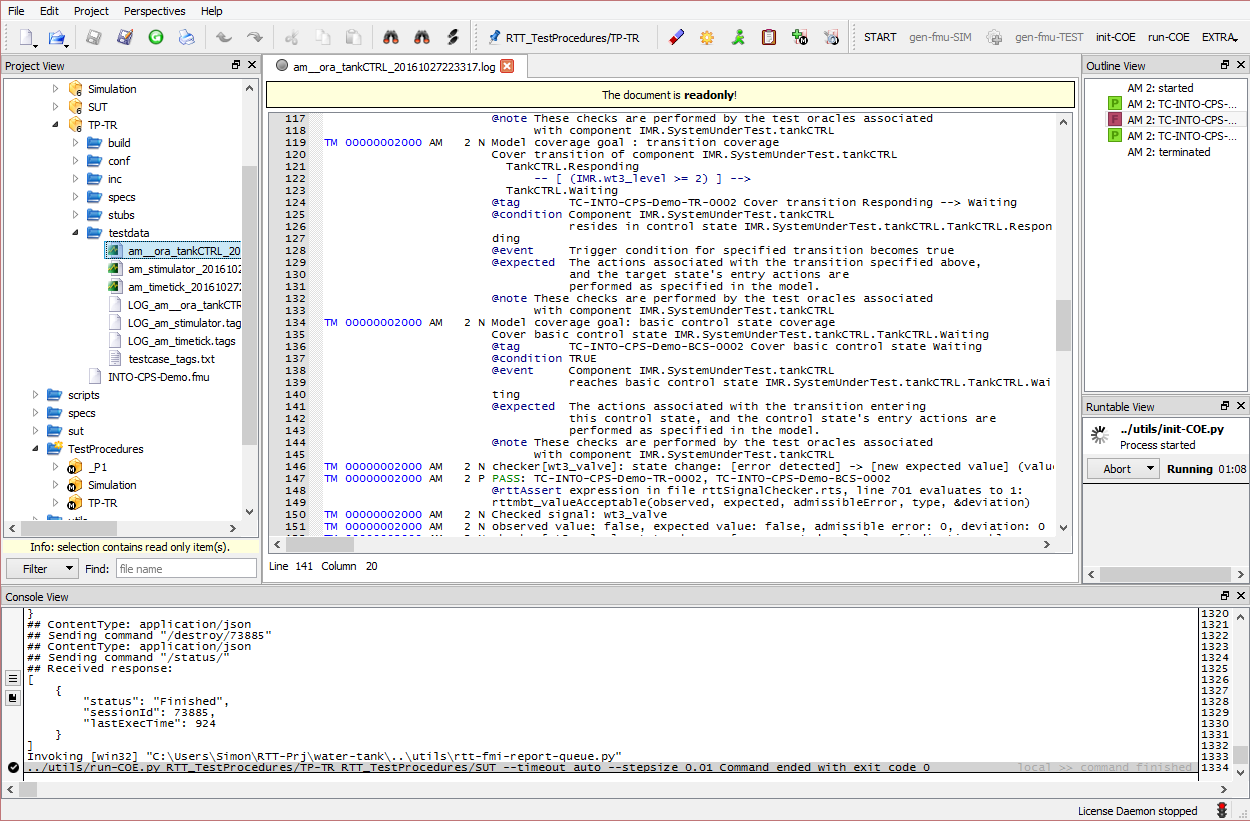
\includegraphics[width=16cm]{threetank/ta_rtt1.png}
  \end{center}
  \caption{Test procedure output}
  \label{fig:ta-out}
\end{figure}


The project can then be prepared for executing the tests through the \emph{init-Project} command that creates the test
FMUs. Finally, the test procedure can be executed by starting the COE, and then using the \emph{run-COE} command. This
will produce output which is exemplified in Figure~\ref{fig:ta-out}.

\subsubsection{Code Generation}

The VDM-RT model, \textbf{WaterTankController} can be exported from Overture as a C code FMU, in addition to the tool wrapper FMU as used above. The \emph{WaterTankController-SourceCode.FMU} included in this pilot is obtained directly from Overture using the ``Export Source Code FMU'' option. However, this FMU does not contain binaries for co-simulation and so one may use the \emph{FMU Builder} included in the INTO-CPS Application to compile FMUs for Windows, Mac and Linux. 

This process has been performed and the resultant FMU is included in the pilot in the FMUs folder; \emph{WaterTankController-Standalone.FMU}. One example experiment available is to switch this FMU for the tool wrapper version -- \emph{WaterTankController.FMU} -- and compare results. 